\chapter[Conclusions and Future Work]{Conclusions and Future Work}
\label{chap:Conclusions}

%=====================================================================================================
\section{Conclusions}
\label{conclusions}



%=====================================================================================================
\section{Contributions}
\label{contributions}

This dissertation has the following contributions to Computer Science research.

\begin{itemize}
\item Identified attributes scale table. Serves as guideline in autonomous component design and autonomy management tools.
\item Managing autonomy by managing information approach at three scales.
\item 
Designed a Bayesian model

Proposed a heuristic that enabled hierarchical search in parameter space.

Designed multiple path planning algorithms, real-time, partial detection.





%=====================================================================================================
\section{Future Work}
\label{futurework}

%===================================================
\subsection{At the Strategic Scale}

After the searcher provides some initial lost person profile information (such as age, gender, etc.), the system will suggest transitional probability values based on statistics from past incidents~\cite{Koester2008Lost}. The searcher can use the suggested parameters or specify them manually using the proposed information management tool, \textbf{ParamMod}. Figure~\ref{Mockup1} shows a mock up screen of the \textbf{ParamMod} tool. A searcher can move two sliders to set the mean and standard deviation of a Beta distribution and see immediately how the shape of the Beta distribution would change respectively. We use mean and standard deviation parameters because they are easy to understand (in contrast to the $\alpha$ and $\beta$ parameters in the Beta distribution function). As the searcher changes the shape of each transitional probability distribution, the searcher will also see immediately how the changes affect the final 3D probability distribution map. This immediate visual feedback allows the user to understand causal effects and therefore helps the user form a mental model of the system that is similar to how the system truly works. Computationally, instant feedback requires that we perform matrix computations on the GPU using CUDA (Compute Unified Device Architecture) architecture. We have been collaborating with Mike Roscheck to implement this and will publish a paper on it.

\begin{figure}
\centering
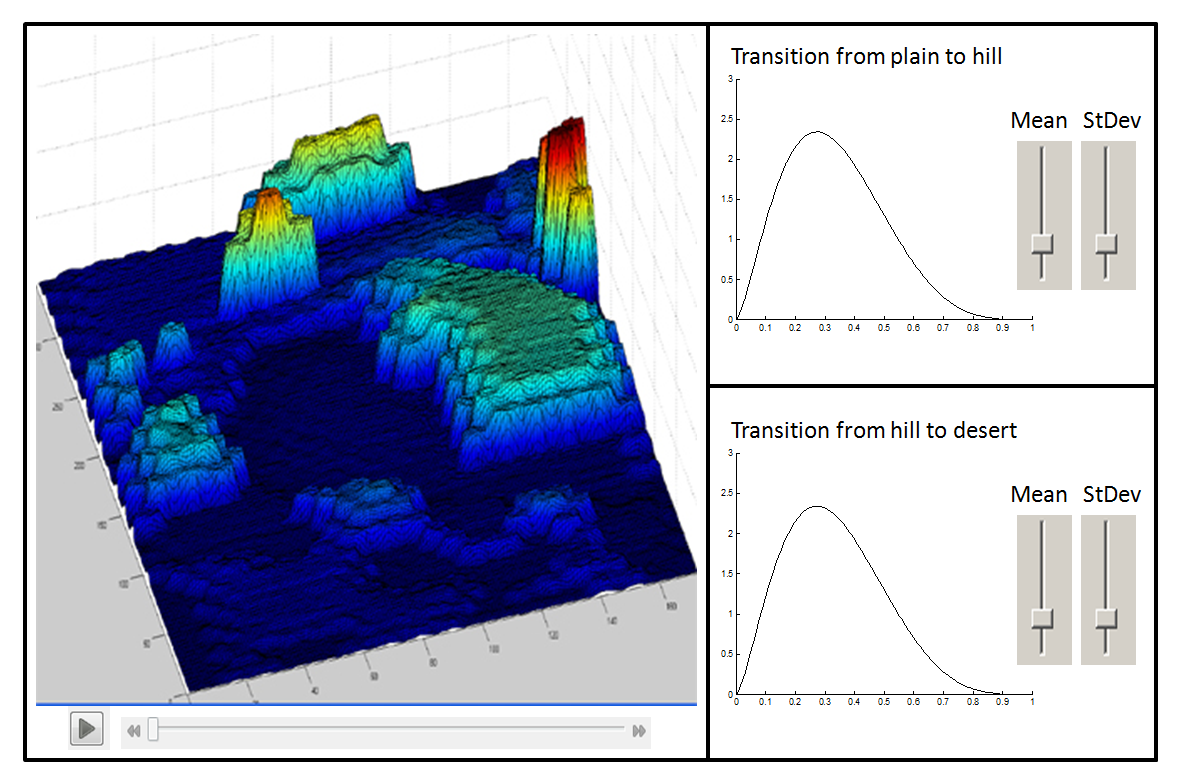
\includegraphics[width=3in]{Mockup1.png}
\caption{A mock up screen for the management tool interface at the general trend scale.}
\label{Mockup1}
\end{figure}

Comparing the prior predictive to the posterior predictive distribution should allow the searcher to understand the causal relationship of how the decision affects the probability distribution map produced. We plan to use selected geocacher GPS track logs downloaded from Everytrail.com as the dataset. We will also create utility tools to process these GPS track logs, including automatically downloading and labeling related terrain features.


%The current Bayesian model uses external calls to MATLAB for large-size matrix multiplications and it takes roughly 4 seconds to multiple two 608 $\times$ 608 matrices. Since one matrix multiplication is needed for each time interval (1 minute), generating a predictive probability distribution for a 3-hour duration would require 180 matrix multiplications, which will take 12 minutes computation time. If after a user changes a model parameter, he/she has to wait 12 minutes to see how the parameter change affects the final product of the model, it is not very useful especially with respect to seeing the causal relationship. We propose to take advantage of powerful GPUs and use the CUDA (Compute Unified Device Architecture) parallel computation architecture developed by NVIDIA to speed up the matrix multiplications. Initial test runs of multiplying two 608 $\times$ 608 matrices on a GeForce GTX480 GPU took only 2 miliseconds. Such speed up enables the user to see immediately how parameter changes could affect the shape of the 3D probability distribution produced by the model. However, the immediate feedback is only avaible when computing the prior preditive probability (without using past human behavior data) because computing the posteriors of the transitional probabilities still takes 220 seconds when using the MCMC algorithm.


%Because intended destination and trail-following behaviors are important factors that can affect a lost person's behavior~\cite{Lin2010Bayesian}, we plan to include them in our \textbf{TBMod} model. Because trail data are not readily available directly from public resources, our utility tools will allow a user to trace trails from an overlaid satellite image of the region and add the topographical feature to the dataset. To add the intended destination feature, we include a prior node in our Bayesian network representing the probability of traveling to different directions with respect to how dispersed the direction is from the intended destination. This prior node will follow a categorical distribution, but the probability of each category is determined by a Gaussian distribution. A scaler parameter $s$ will be used to specify how the Gaussian distribution can be divided into different categories.

%The autonomy interface management tool should allow the searcher to first mark Point Last Seen and intended destination on the terrain map overlay, then specify lost person profile information such as age group and gender,  next choose whether to use past human behavior data, and finally choose whether to specify transitional probabilities manually.

%===================================================
\subsection{At the Between-Episodes Scale}

%===================================================
\subsection{At the Within-Episode Scale}




